\documentclass[10pt, spanish]{beamer}
\usepackage[spanish]{babel}

\usetheme[progressbar=frametitle]{metropolis}

\usepackage{booktabs}
\usepackage[scale=2]{ccicons}

\usepackage{pgfplots}
\usepgfplotslibrary{dateplot}

\usepackage{float}
\graphicspath{ {images/} }

%% COLOR
\usepackage{color, colortbl}
\definecolor{Gray}{gray}{0.9}	
\definecolor{LightCyan}{rgb}{0.88,1,1}

\title{Identificaci\'on de patrones y algoritmos de consolidaci\'on en bases de datos de posicionamiento}
\date{\today}
\author{Pilar Barbero Iriarte}
\institute{Universidad de Zaragoza}
\titlegraphic{\hfill
\includegraphics[height=1.5cm]{unizar.png}}

\begin{document}

\maketitle

\begin{frame}
  \frametitle{Table of Contents}
  \setbeamertemplate{section in toc}[sections numbered]
  \tableofcontents[hideallsubsections]
\end{frame}

\section{Introducci\'on}

%%Introducci\'on
\begin{frame}[fragile]
\frametitle{Introducci\'on}
Contexto: 
\begin{itemize}
	\item Empresa Zaragozana de telecomunicaciones.
	\item Almacenamiento de posiciones GPS de sujetos.
	\item Capacidad de guardado de posiciones limitada.
\end{itemize}
\end{frame}


\begin{frame}[fragile]
\frametitle{Introducci\'on}
Problemas:
	\begin{itemize}
		\item Exceso de \'estas.
		\item No existe preprocesado antes de la inserci\'on.
		\item No existe postprocesado despu\'es de la inserci\'on.
		\item No todas aportan informaci\'on.
	\end{itemize}
\end{frame}

%%OBJETIVO
\begin{frame}[fragile]
  \frametitle{Introducci\'on}
  Objetivo:
  \begin{itemize}
  	  \item Eliminar posiciones repetidas.
  	  \item Eliminar posiciones que no aporten informaci\'on.
   \end{itemize}
\end{frame}

\section{An\'alisis de los datos}


\begin{frame}[fragile]
\frametitle{An\'alisis de los datos}
  \begin{itemize}[<+- | alert@+>]    
\item \textbf{Id}: Identificador num\'erico
\item \textbf{IdServidor}: Identificador num\'erico del servidor que realiza la inserci\'on
\item \textbf{Recurso}: identificador del sujeto que transfiere la posici\'on
\item \textbf{Latitud}: real que representa la latitud GPS
\item \textbf{Longitud}: real que representa la longitud GPS
\item \textbf{Velocidad}: entero que representa la velocidad instant\'anea
\item \textbf{Orientaci}\'on: entero que representa la orientaci\'on respecto al norte en grados
\item \textbf{Cobertura}: booleano que indica si tiene cobertura (n. sat\'elites)
\item \textbf{Error}: error en la toma de posici\'on
  \end{itemize}
\end{frame}

\section{¿C\'omo abordar el problema?}
\begin{frame}[fragile]
\frametitle{¿C\'omo abordar el problema?}
\begin{itemize}

\item Desarrollo de algoritmos de consolidaci\'on a trav\'es de nociones de distancia y tiempo.

\item Uso de algoritmos de \textit{clustering} con el fin de identificar varias posiciones con su centro del cl\'uster y consolidarlas en \'esta.

\end{itemize}


\end{frame}


\subsection{M\'etodos simples}
\begin{frame}[fragile]
\frametitle{Consolidaci\'on por distancia}
\end{frame}

\begin{frame}[fragile]
\frametitle{Consolidaci\'on por adelgazamiento}
\end{frame}

\begin{frame}[fragile]
\frametitle{Consolidaci\'on por tiempo}
\end{frame}

\subsection{M\'etodos avanzados}
\begin{frame}[fragile]
\frametitle{K-means}
\end{frame}

\begin{frame}[fragile]
\frametitle{DBSCAN}
\end{frame}

\begin{frame}[fragile]
\frametitle{DJ-Cl\'uster}
\end{frame}


\section{Comparativa casos estudiados}
\begin{frame}[fragile]
\frametitle{Comparativa t\'ecnicas clustering}
\begin{center}
\begin{tabular}{|l|l|l|l|}
	\hline
	\rowcolor{Gray}
	M\'etodo & Tiempo & N. & Iteraciones\\
	\hline	
	K-means & 0.69 secs & 500 & 9\\
	\hline
	DBSCAN &  2 min 30 secs & 9 & 111 \\
	\hline
	DJ-Cluster &  0.37 secs & 22  & 11\\
	\hline
\end{tabular}
\end{center}

\begin{itemize}
	\item DBSCAN m\'as lento de todos.
	\item DBSCAN consolidaci\'on mayor.
	\item K-means se queda en 500 cl\'usters.
	\item DJ-Cl\'uster baja de los 500.
	\item DJ-Cl\'uster menor tiempo de ejecuci\'on.
\end{itemize}

\end{frame}

\begin{frame}[fragile]
\frametitle{Comparativa t\'ecnicas simples}

\begin{center}
\begin{tabular}{|l|l|l|}
	\hline
	\rowcolor{Gray}
	M\'etodo & Tiempo & N. \\
	\hline	
	Cons. por adelgazamiento &  <0.01 sec & 800 \\
	\hline 
	Cons. por distancia simple &  <0.01 sec & 507 \\
	\hline
	Cons. por distancia $t_0-$alcanzable  &  <0.01 sec  & 21\\
	\hline
	Cons. por tiempo &  <0.01 sec  & 1786\\
	\hline
\end{tabular}
\end{center}

\begin{itemize}
	\item Alternar distintos tipos de consolidaci\'on en funci\'on del espacio cr\'itico en ese momento.
\end{itemize}
\end{frame}

\section{Conclusiones}
\begin{frame}[fragile]
\begin{itemize}[<+- | alert@+>]
	\item Algoritmos de consolidaci\'on simples son \textit{simples}, pero eficaces.
	\item Noci\'on de vecindario distinto al eucl\'ideo implementada en algoritmos de consolidaci\'on simple.
	\item Algoritmos de \textit{clustering} m\'as avanzados, pero m\'as complejos a la hora de implementar.
	\item Importante un procesado previo.
	\item A la hora de recuperar una traza con los datos borrados, mejor \textit{DJ-Cl\'uster}
	\item Noci\'on de ruido de DBSCAN importante, tanto DJ-Cl\'uster como K-means s\'olo encuentra cl\'usters de tama\~no 1.
\end{itemize}
\end{frame}

\section{Demostraci\'on}

\section{Preguntas}

\begin{frame}[fragile]
	\frametitle{C\'odigo}
	\begin{center}
		\href{http://github.com/pbarbero/TFM}{http://github.com/pbarbero/TFM}
		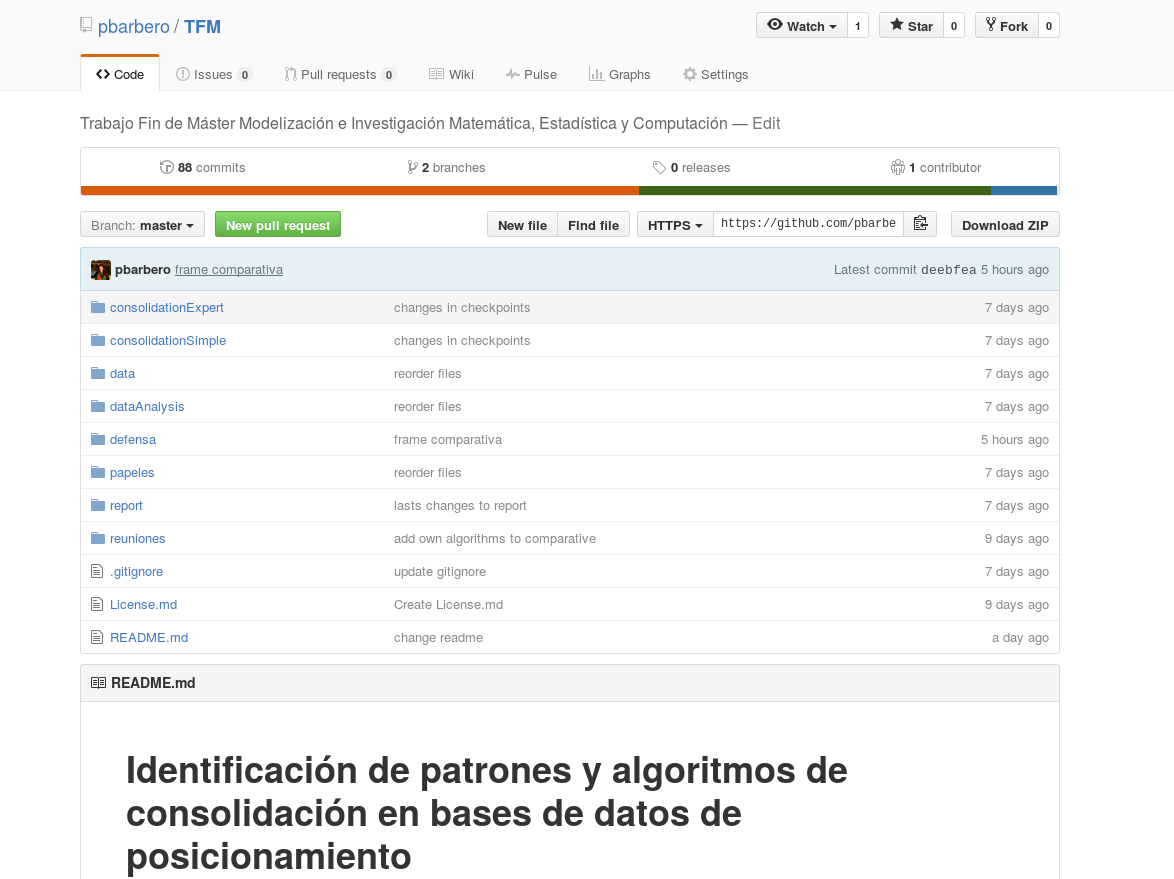
\includegraphics[scale=.3]{github.png}
	\end{center}
\end{frame}

\end{document}
